\def\objectdetectionhighres{
    \section{Các mô hình giải quyết bài toán Object Detection trong ảnh chất lượng cao}
    \subsection{Các thí nghiệm về tỷ lệ giữa kích thước của đối tượng trong ảnh và kích thước ảnh}
    Trước khi bàn luận đến những mô hình giúp giải quyết bài toán Object Detection trong ảnh chất lượng cao, 
    ta cần xem xét đến vai trò của tỷ lệ giữa kích thước của đối tượng trong ảnh và kích thước ảnh thông qua một số thí nghiệm.
    Cụ thể hơn, nhóm tác giả muốn đánh giá sự ảnh hưởng \textit{domain shift}
    (\textit{domain shift} ở đây được định nghĩa là sự chuyển dịch về tỷ lệ giữa kích thước của đối tượng trong ảnh và kích thước ảnh giữa tập dữ liệu train và tập dữ liệu test) 
    lên kết quả của mô hình.
    \textit{Domain shift} rất phổ biến trong bài toán Object Detection, khi kích thước ảnh sử dụng trong quá trình train thường nhỏ (nhằm cải thiện tốc độ train mô hình) và
    kích thước ảnh sử dụng trong quá trình test thường lớn hơn để cải thiện kết quả với những object nhỏ trong ảnh.
    Các thí nghiệm này được xây dựng và công bố kết quả bởi Bharat Singh và các cộng sự với mô hình SNIP \cite{singh2018analysis}.
    \subsubsection{Các thí nghiệm trong bài toán Image Classification}
    Trước khi tiến hành các thí nghiệm với bài toán Object Detection,
    nhóm tác giả đã thực hiện các thí nghiệm với bài toán Image Classification vì
    đây là một bài toán cơ bản, phổ biến và cũng là một bài toán con trong bài toán Object Detection. \\
    
    \noindent
    \textbf{\textit{Cấu hình của các mô hình trong các thí nghiệm}} \\
    Ba mô hình được sử dụng trong các thí nghiệm được thiết kế như sau:
    \begin{figure}[H]
        \centering
        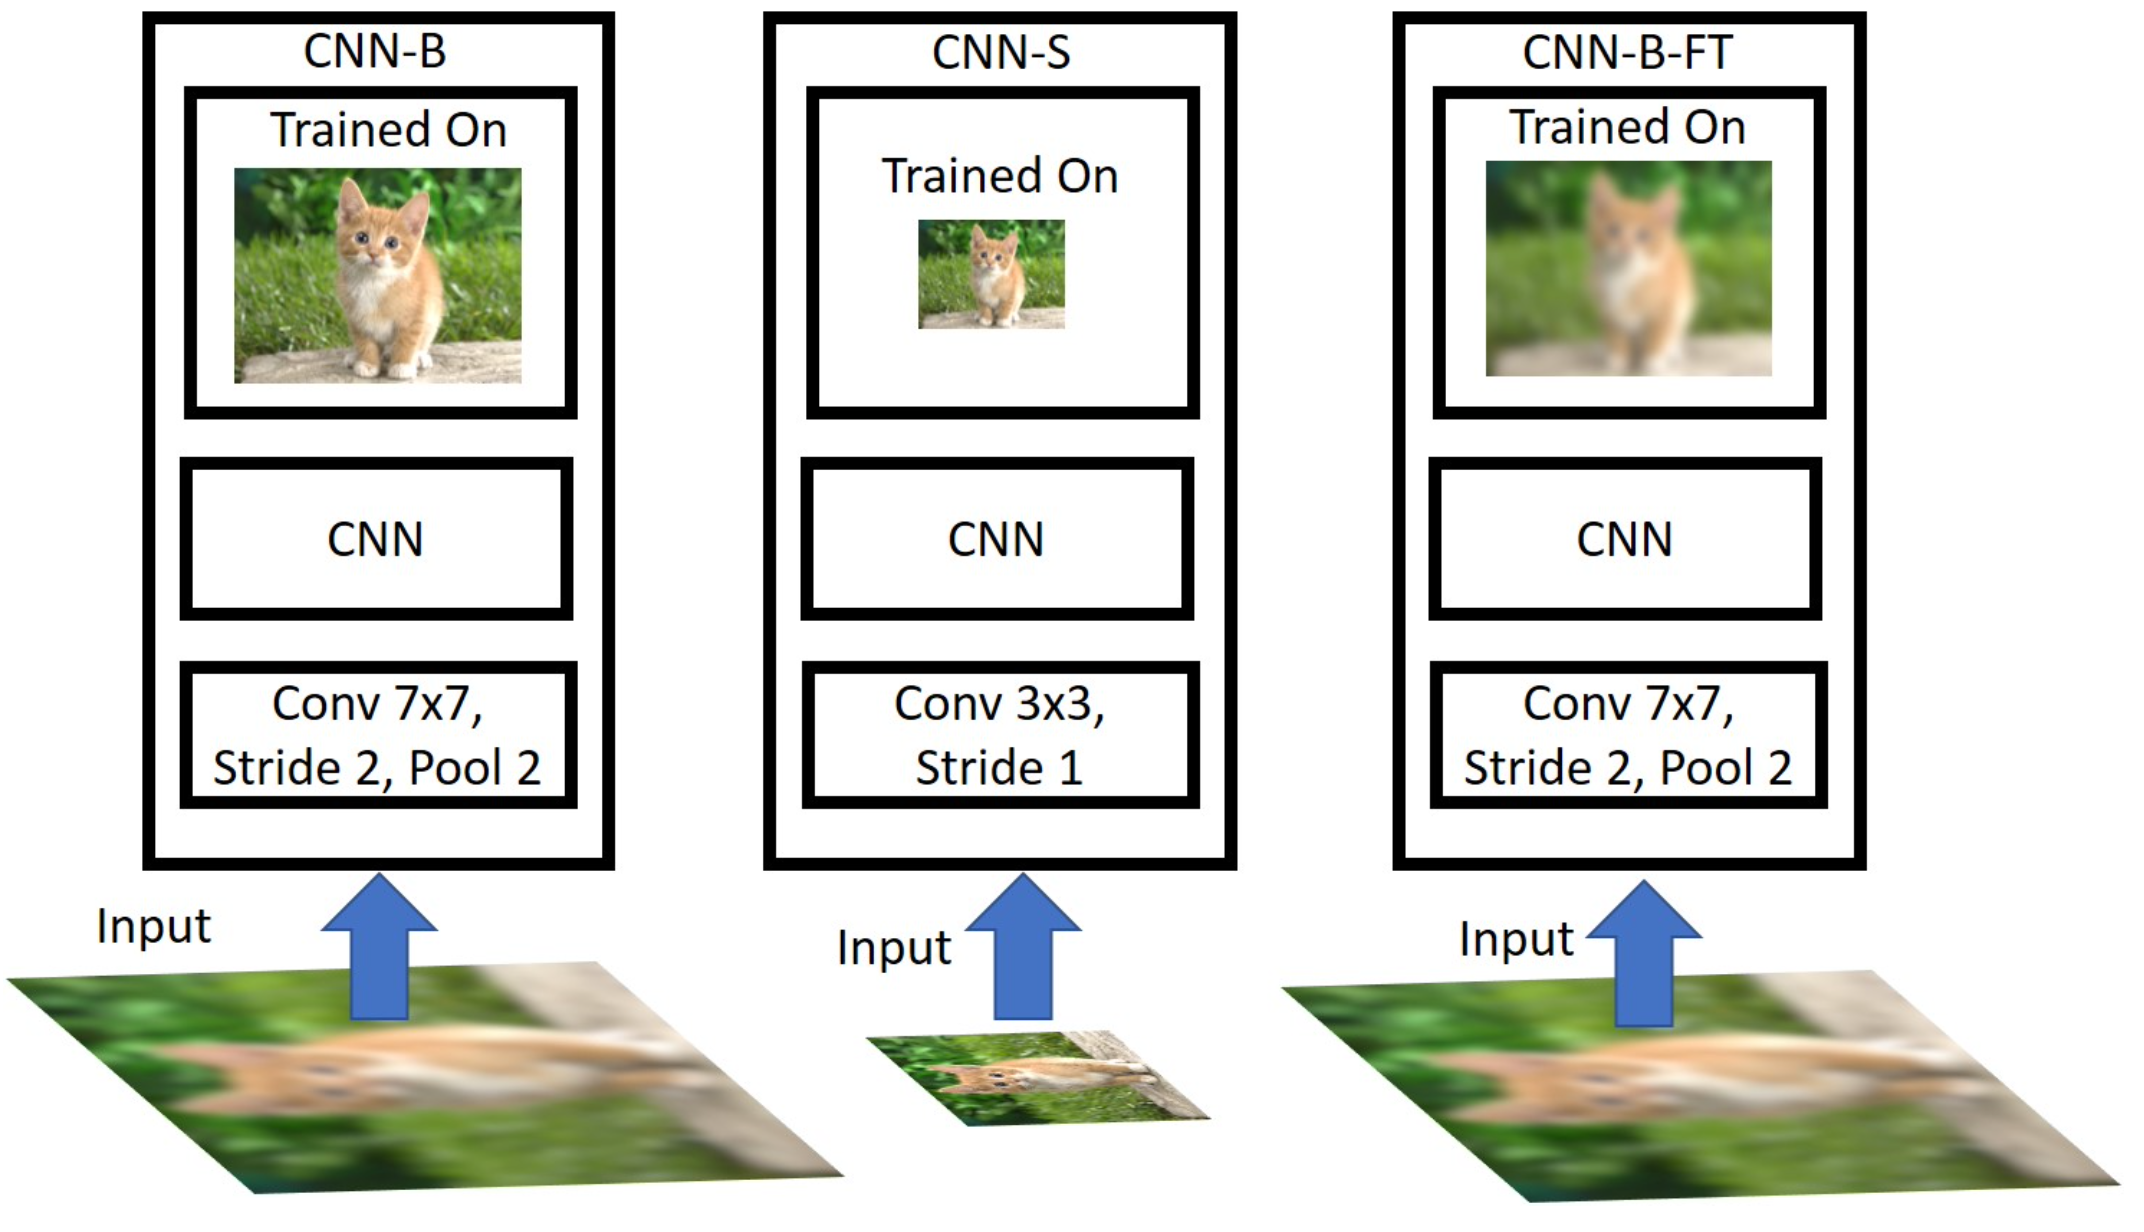
\includegraphics[width=12cm] {images/snip_models_to_exp.png}
        \caption{Ba mô hình được sử dụng trong các thí nghiệm (Nguồn: \cite{singh2018analysis})}
        \label{fig:snip_models_to_exp}
    \end{figure}
    
    \noindent
    - Mô hình CNN-B: Đây là mô hình CNN sử dụng backbone ResNet-101 và đã được train với bộ dữ liệu ảnh có kích thước 224x224. \\
    - Mô hình CNN-S: Đây là mô hình CNN sử dụng backbone ResNet-101 và đã đã được thay đổi các tham số stride và kích thước của conv trong lớp đầu tiên đối với từng bộ dữ liệu ảnh có kích thước khác nhau khi train mô hình.
    Khi train với bộ dữ liệu ảnh có kích thước 48x48, tác giả dùng conv có kích thước 3x3 và stride bằng 1,
    khi train với bộ dữ liệu ảnh có kích thước 96x96, tác giả dùng conv có kích thước 5x5 và stride bằng 2. \\
    - Mô hình CNN-B-FT: Đây là mô hình CNN sử dụng backbone ResNet-101 và đã được train với bộ dữ liệu ảnh có kích thước 224x224 giống như CNN-B. Sau đó fine-tune lại với bộ dữ liệu ảnh có kích thước nhỏ hơn nhưng được upsample lên lại kích thước 224x224. \\

    \noindent
    \textbf{\textit{Thí nghiệm Naive Multi-Scale Inference}} \\
    Nhóm tác giả kiểm tra đánh giá mô hình CNN-B đơn giản với các bộ dữ liệu có kích thước ảnh khác nhau.
    Đầu tiên, nhóm tác giả thu nhỏ kích thước ảnh trong bộ dữ liệu ImageNet từ 224x224 xuống 48x48, 64x64, 80x80, 96x96, 128x128.
    Tiếp theo, nhóm tác giả tăng kích thước ảnh từ 48x48, 64x64, 80x80, 96x96, 128x128 lên lại 224x224.
    Cuối cùng, với các bộ dữ liệu mới nói trên, nhóm tác giả đưa vào mô hình CNN-B và quan sát kết quả. \\
    \textbf{Kết quả}: Ảnh sử dụng trong quá trình train và trong quá trình test càng khác nhau về kích thước, khả năng của mô hình càng giảm.
    Cụ thể hơn, kết quả về top-1 accuracy của mô hình CNN-B với các bộ dữ liệu được tăng kích thước từ 48x48, 64x64, 80x80, 96x96, 128x128 lần lượt là 33.8\%, 45.8\%, 53.8\%, 59.7\%, 67.1\%.
    Trong khi đối với bộ dữ liệu được giữ nguyên kích thước 224x224, mô hình CNN-B đạt kết quả 76.8\%.

    \begin{figure}[H]
        \centering
        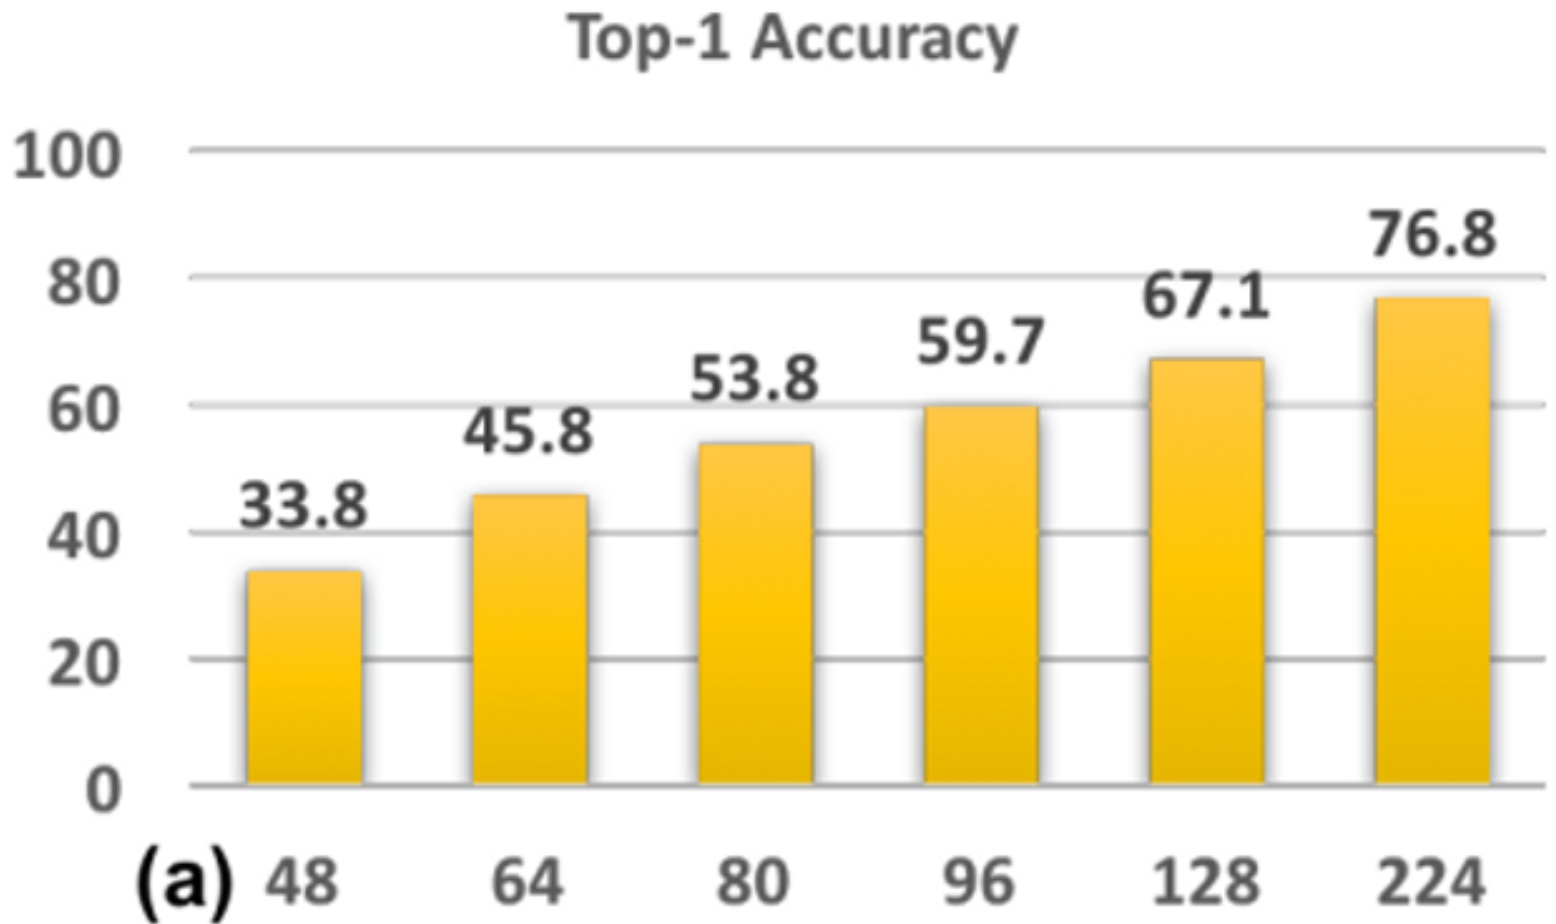
\includegraphics[width=9cm] {images/snip_naive_multi_scale_infer}
        \caption{Kết quả của thí nghiệm Naive Multi-Scale Inference (Nguồn: \cite{singh2018analysis})}
        \label{fig:snip_naive_multi_scale_infer}
    \end{figure}

    \noindent
    \textbf{Kết luận}: Đối với bài toán classification, việc test mô hình với các kích thước ảnh khác mà mô hình chưa được train sẽ gây ra kết quả suy giảm đáng kể.
    Sự chênh lệch càng lớn giữa kích thước ảnh train và kích thước ảnh test càng gây ra sự suy giảm kết quả đáng kể. \\

    \noindent
    \textbf{\textit{Thí nghiệm Resolution Specific Classifiers}} \\
    Trong thí nghiệm này, nhóm tác giả thay đổi một chút kiến trúc của mô hình CNN-S.
    Trong kiến trúc của mô hình CNN-B, lớp conv đầu tiên có kích thước stride = 2, và sau đó là lớp max pooling với stride = 2x2.
    Do đó, ngay từ các lớp đầu tiên, các mô hình trên xoá đi các thông tin của các đối tượng nhỏ trong ảnh.
    Từ quan sát trên, nhóm tác giả thay đổi kiến trúc và tạo ra mô hình CNN-S sao cho nó đạt được kết quả tốt nhất trên bộ CIFAR10 (đây là bộ dữ liệu với kích thước ảnh nhỏ).
    Sau đó, nhóm tác giả so sánh kiến trúc của mô hình CNN-S với mô hình CNN-B. \\
    \textbf{Kết quả}: Mô hình CNN-S đạt kết quả tốt hơn rất nhiều so với kết quả của mô hình CNN-B khi xử lý ảnh 48x48.
    Trong khi mô hình CNN-B đạt kết quả 33.8\%, mô hình CNN-S đạt kết quả 60.38\%. \\
    \textbf{Kết luận}: Việc thay đổi kiến trúc của mô hình sao cho phù hợp giúp cho mô hình học ảnh có resolution nhỏ tốt hơn.

    \begin{figure}[H]
        \centering
        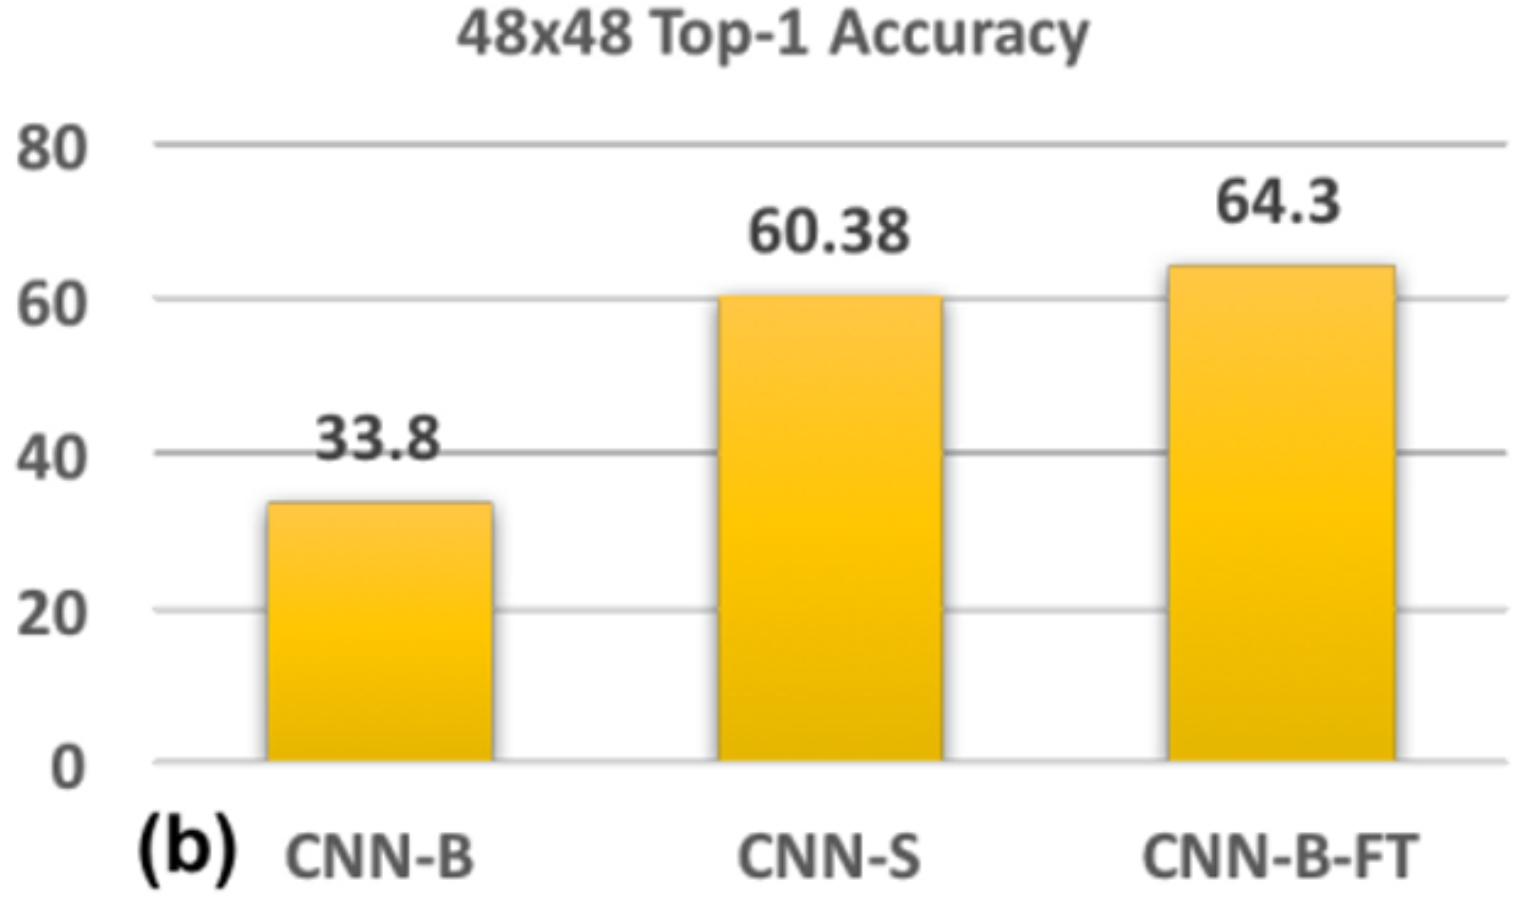
\includegraphics[width=9cm] {images/snip_res_spec_cls}
        \caption{Kết quả của thí nghiệm Resolution Specific Classifiers và Fine-tuning High-Resolution Classifiers trên bộ dữ liệu ảnh có kích thước 48x48 (Nguồn: \cite{singh2018analysis})}
        \label{fig:snip_res_spec_cls}
    \end{figure}

    \noindent
    \textbf{\textit{Thí nghiệm Fine-tuning High-Resolution Classifiers}} \\
    Việc thiết kế và train mô hình (tương như như phương án của mô hình CNN-S trong thí nghiệm Resolution Specific Classifiers) với mỗi một bộ dữ liệu có kích thước ảnh khác nhau sẽ tốn quá nhiều công sức và tài nguyên tính toán.
    Từ đó, nhóm tác giả đưa ra một giải pháp đơn giản hơn đó là chiến lược xây dựng mô hình CNN-B-FT. \\
    \textbf{Kết quả}: Mô hình CNN-B-FT có kết quả tốt hơn so với kết quả của mô hình CNN-S. \\
    \textbf{Kết luận}: Thí nghiệm trên chứng minh rằng, các trọng số của mô hình CNN-B, được train từ bộ dữ liệu ảnh có kích thước lớn, hữu ích trong việc giải quyết bộ dữ liệu ảnh có kích thước nhỏ.
    Từ đó, thay vì giảm kích thước stride của lớp conv đi 2 lần (như trong kiến trúc của mô hình CNN-S), ta nên tăng kích thước của ảnh chất lượng thấp lên lần và fine-tune lại với mô hình đã được train với bộ dữ liệu ảnh có kích thước lớn.
    Hay nói cách khác, thay vì thay đổi kiến trúc của mô hình để xử lý riêng với bộ dữ liệu ảnh có kích thước nhỏ, ta nên tận dụng mô hình pretrained và fine-tune lại mô hình đó với bộ dữ liệu ảnh có kích thước mong muốn.

    \begin{figure}[H]
        \centering
        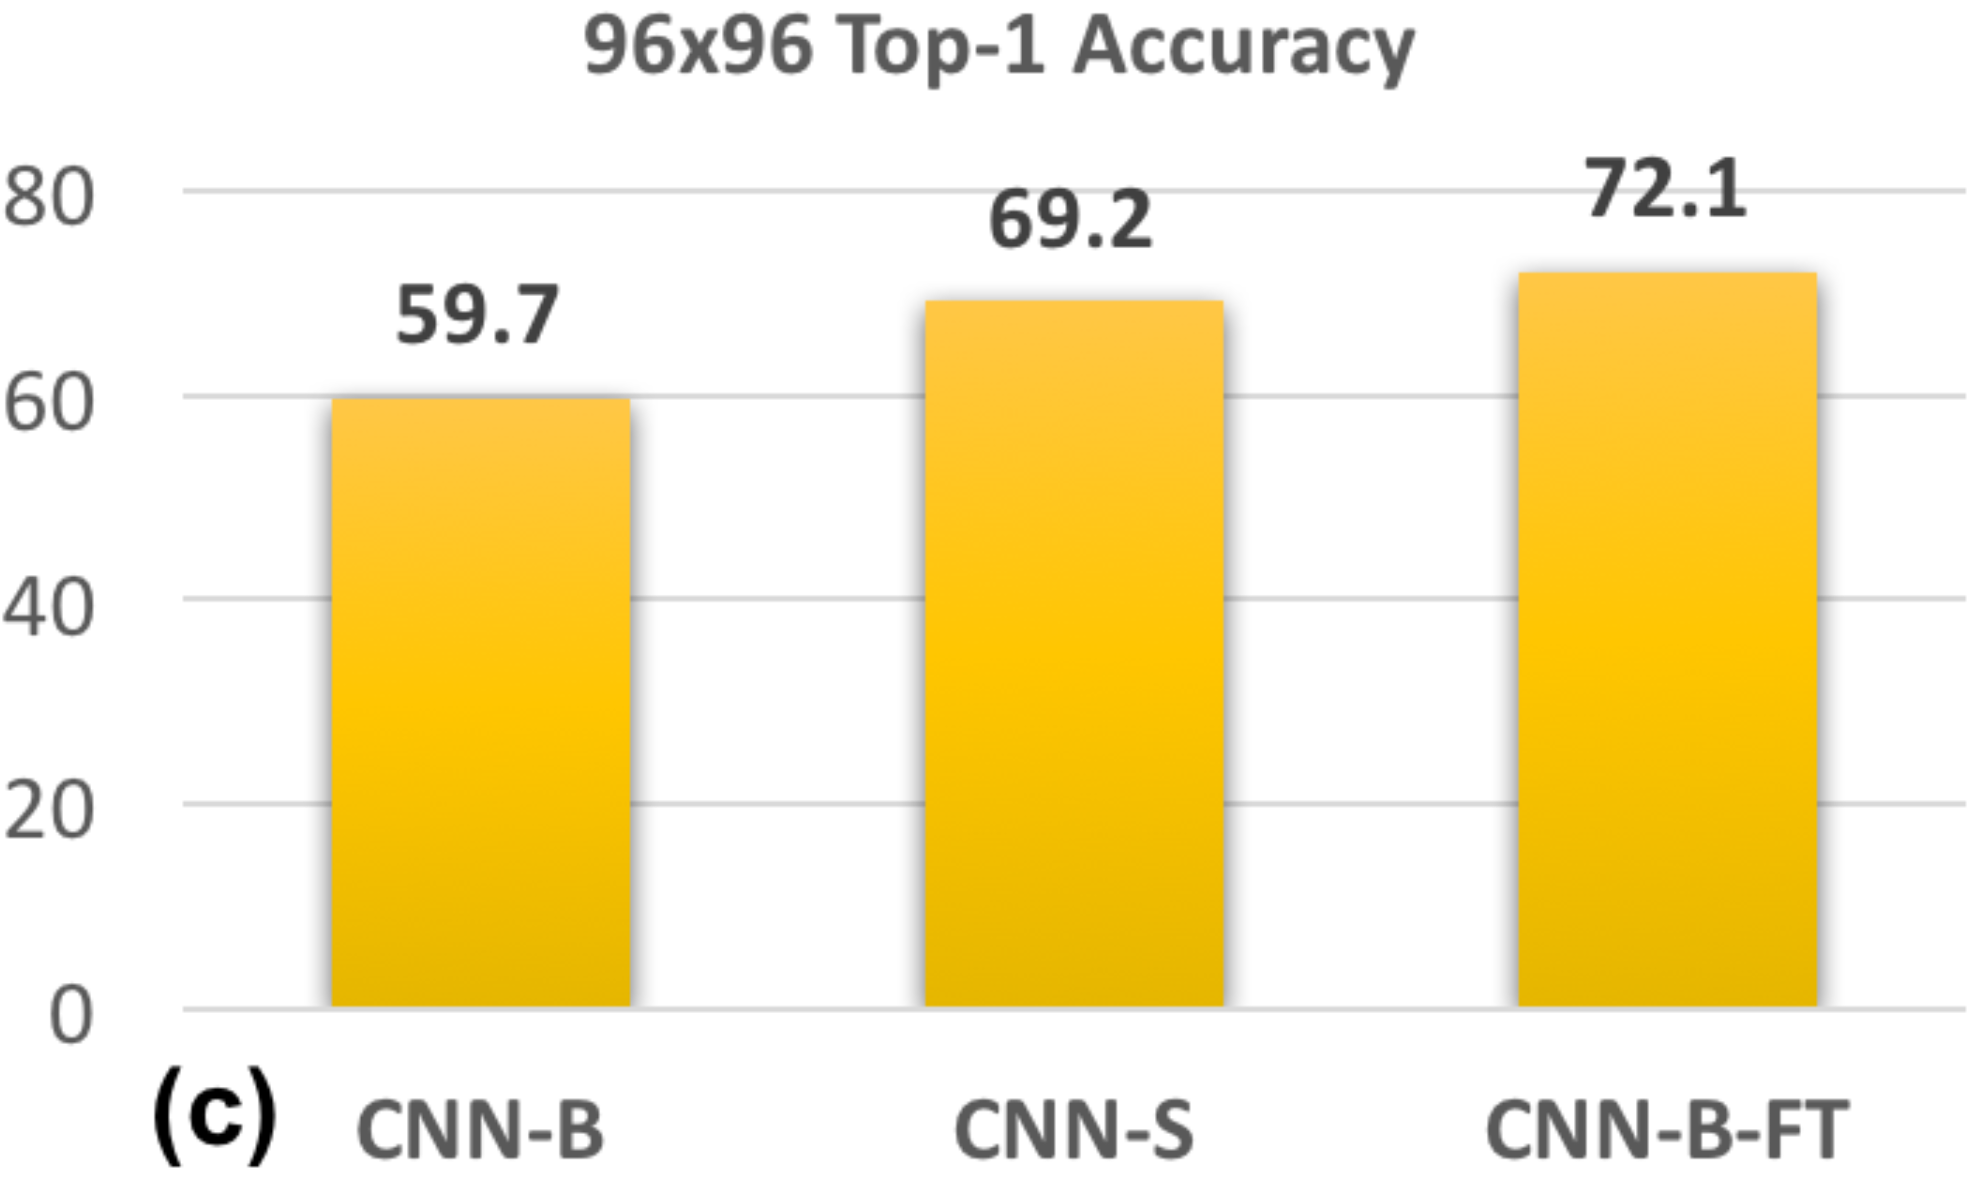
\includegraphics[width=9cm] {images/snip_res_spec_cls_96}
        \caption{Kết quả của thí nghiệm Resolution Specific Classifiers và Fine-tuning High-Resolution Classifiers trên bộ dữ liệu ảnh có kích thước 96x96 (Nguồn: \cite{singh2018analysis})}
        \label{fig:snip_res_spec_cls_96}
    \end{figure}

    \subsubsection{Các thí nghiệm trong bài toán object detection}
    Hiệu năng giữa các mô hình bị ảnh hưởng bởi sự khác nhau về kích thước của ảnh trong bộ dữ liệu train và bộ dữ liệu test đã được nhóm tác giả chứng minh ở các thí nghiệm trên.
    Tuy nhiên, trong thực tế, không phải lúc nào ta cũng có thể train và test mô hình với bộ dữ liệu ảnh có cùng kích thước, đặc biệt đối với bài toán Object Detection.
    Lý do vì những vấn đề liên quan đến bộ nhớ của GPU cũng như là tốc độ train của mô hình, do đó, thông thường kích thước ảnh trong bộ dữ liệu sử dụng trong quá trình train thường nhỏ hơn so với kích thước ảnh trong quá trình test. \\
    Trong các thí nghiệm ở phần này, nhóm tác giả train các mô hình với các cài đặt khác nhau nhưng cùng test trên bộ dữ liệu có kích thước 1400x2000 nhằm mục đích đánh giá hiệu năng của các mô hình trong việc detect các object nhỏ (kích thước nhỏ hơn 32x32) \\

    \noindent
    \textbf{\textit{Cấu hình của các mô hình trong các thí nghiệm}} \\
    TODO: ádsad Phần 4 trong paper SNIP \\

    \noindent
    \textbf{\textit{Thí nghiệm train các mô hình với kích thước ảnh khác nhau}} \\
    Trong thí nghiệm này, nhóm tác giả train hai mô hình với hai bộ dữ liệu lần lượt có kích thước ảnh là 800x1400 và 1400x2000 (tác giả gọi hai mô hình lần lượt là mô hình ${800}_{all}$ và mô hình ${1400}_{all}$).
    Và toàn bộ các object của cả hai bộ dữ liệu này đều được sử dụng để train mô hình. \\
    \textbf{Kết quả}: Hiển nhiên, mô hình ${1400}_{all}$ hoạt động tốt hơn so với mô hình ${800}_{all}$.
    Tuy nhiên, phần hơn của mô hình ${1400}_{all}$ là chưa đáng kể. \\
    \textbf{Kết luận}: Việc train mô hình ${1400}_{all}$ với ảnh có kích thước lớn hơn giúp các object nhỏ được tăng kích thước so với mô hình ${800}_{all}$, từ đó, các object này được train một cách dễ dàng hơn.
    Nhưng ở chiều ngược lại, những object trung bình và lớn trong ảnh cũng bị tăng kích thước theo khiến cho chúng trở nên quá lớn và trở nên khó khăn cho mô hình ${1400}_{all}$ có thể học một cách chính xác.
    Lượng dữ liệu khó học từ object trung bình và lớn này khiến cho mô hình ${1400}_{all}$ không thể vượt trội so với mô hình ${800}_{all}$. \\

    \noindent
    \textbf{\textit{Thí nghiệm train mô hình với các object có kích thước cụ thể}} \\
    Trong thí nghiệm này, nhóm tác giả vẫn train mô hình với bộ dữ liệu có kích thước 1400x2000.
    Tuy nhiên, nhóm tác giả loại bỏ hoàn toàn các object trung bình và lớn (các object có kích thước lớn hơn 80 trong ảnh gốc) và gọi đây là mô hình ${1400}_{<80px}$ \\
    \textbf{Kết quả}: Kết quả của mô hình ${1400}_{<80px}$ rất tệ so với kết quả của mô hình ${800}_{all}$ và ${1400}_{all}$. \\
    \textbf{Kết luận}: Việc loại bỏ hoàn toàn các object trung bình và lớn khiến cho lượng dữ liệu mà mô hình ${1400}_{<80px}$ được học giảm đi rất nhiều so với các mô hình trên (giảm khoảng 30\% lượng object).
    Từ đó, khi không được học nhiều biến thể của object, kết quả của mô hình ${1400}_{<80px}$ bị ảnh hưởng nghiêm trọng.
    Chúng ta cũng có thể rút ra được một kết luận là, cho dù các mô hình ${1400}_{all}$ và ${800}_{all}$ không hoàn toàn học được các object trung bình và lớn nhưng lượng dữ liệu từ các object này vẫn đóng vai trò quan trọng trong việc giúp mô hình detect các object nhỏ. \\

    \begin{figure}[H]
        \centering
        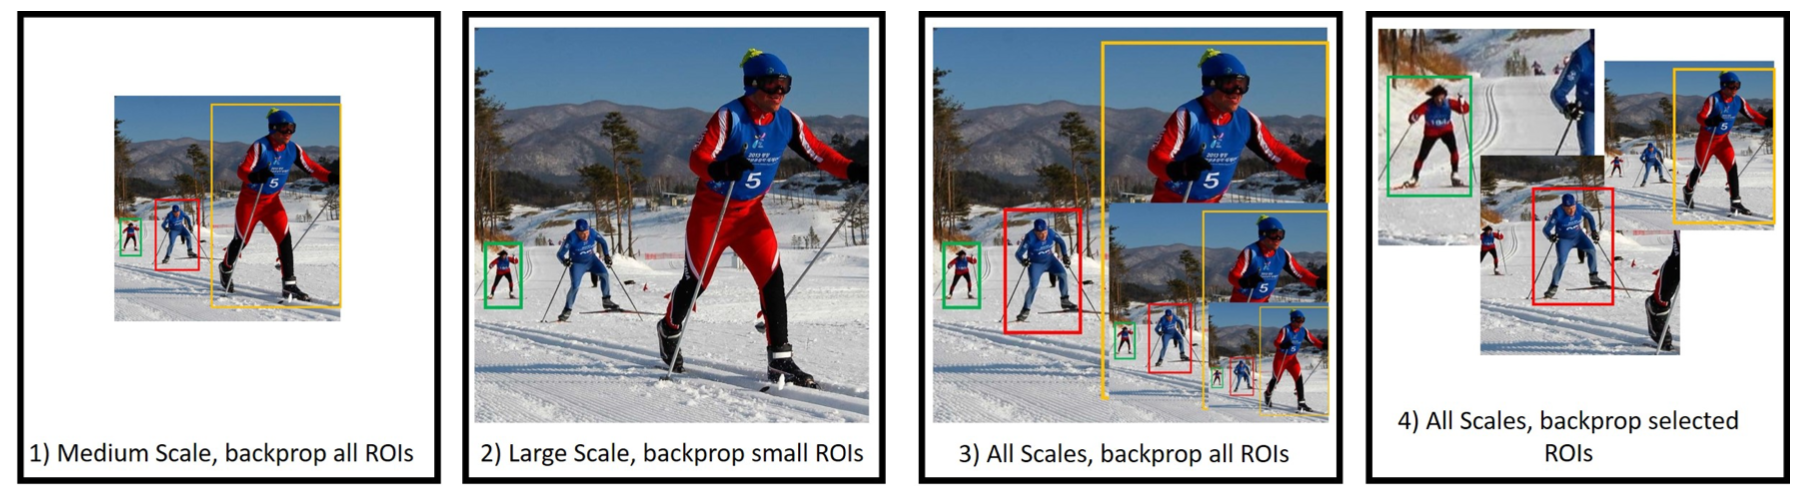
\includegraphics[width=15cm] {images/snip_model_compare}
        \caption{Các cách train mô hình khác nhau 1. ${800}_{all}$, 2. ${1400}_{<80px}$, 3. MST, 4. SNIP (Nguồn: \cite{singh2018analysis})}
        \label{fig:snip_model_compare}
    \end{figure}

    \noindent
    \textbf{\textit{Thí nghiệm train với bộ dữ liệu ảnh có các kích thước khác nhau}} \\
    Nhóm tác giả thực hiện thí nghiệm train mô hình bộ dữ liệu ảnh có các kích thước khác nhau được lựa chọn ngẫu nhiên trong suốt quá trình train (Multi-Scale Training) và mô hình này được gọi là mô hình MST.
    Thí nghiệm này giúp mô hình có thể được học các kích thước khác nhau với mỗi object trong bộ dữ liệu. \\
    \textbf{Kết quả}: Kết quả của mô hình MST xấp xỉ so với kết quả của mô hình ${800}_{all}$. \\
    \textbf{Kết luận}: Việc train mô hình MST với dữ liệu ảnh có các kích thước khác nhau trong suốt quá trình khiến mô hình này gặp khó khăn trong việc học các object rất lớn hoặc rất nhỏ.
    Điều này phần nào đó tương tự với hiện tượng mà mô hình ${1400}_{all}$ gặp phải.

    \begin{figure}[H]
        \centering
        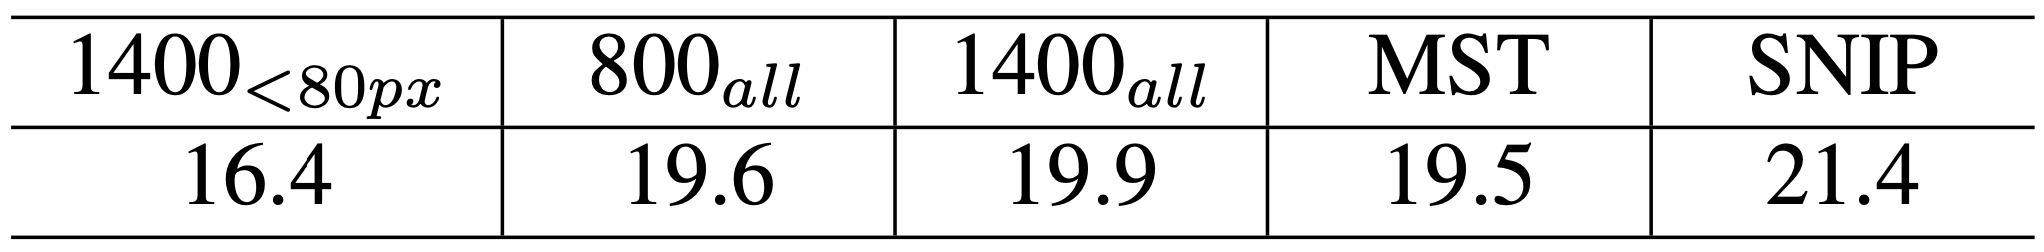
\includegraphics[width=13cm] {images/snip_result_compare}
        \caption{So sánh kết quả trên chỉ số mAP của các mô hình ${1400}_{<80px}$, ${800}_{all}$, ${1400}_{all}$, MST và SNIP trên các object có kích thước nhỏ (nhỏ hơn 32x32) (Nguồn: \cite{singh2018analysis})}
        \label{fig:snip_result_compare}
    \end{figure}

    \subsection{Mô hình SNIP}
    Từ những thí nghiệm trên, nhóm tác giả đã đưa ra đề xuất mô hình Scale Normalization for Image Pyramids (gọi tắt là SNIP) \cite{singh2018analysis}.
    Mô hình SNIP hướng đến việc sử dụng tối đa sự đa dạng trong biến thể của object trong bộ dữ liệu trong khi có thể thu hẹp được sự biến động trong kích thước của các object.
    Từ đó, mô hình sẽ có nhiều dữ liệu nhất có thể và cũng sẽ có kích thước object phù hợp nhất để học.
    Ngoài ra, ý tưởng của mô hình SNIP cũng sẽ giúp train mô hình với Image Pyramid.
    Tương tự như Feature Pyramid, Image Pyramid là ý tưởng về việc sử dụng cùng một ảnh với các kích thước khác nhau nhằm khai thác tối đa thông tin của một ảnh.

    \subsubsection{Ý tưởng của mô hình SNIP}
    Một điểm yếu của mô hình MST ở thí nghiệm trên là việc một ảnh bất kỳ được train với nhiều kích thước khác nhau khiến cho khi ảnh đó ở kích thước lớn (1400x2000) thì các object lớn sẽ trở nên khó khăn cho mô hình.
    Điều này diễn ra tương tự đối với các object nhỏ khi ảnh đó ở kích thước nhỏ (480x800). \\
    SNIP được coi là một phiên bản tinh chỉnh của MST.
    Ý tưởng chính của SNIP là trong quá trình train, các object có kích thước tương đồng với bộ dữ liệu pretrained của mô hình (thông thường là 224x224) sẽ được sử dụng để train.
    Nhằm tránh gặp phải vấn đề như  MST, SNIP loại bỏ các object, mà sau khi thay đổi kích thước ảnh, trở nên quá lớn hoặc quá nhỏ.
    \begin{figure}[H]
        \centering
        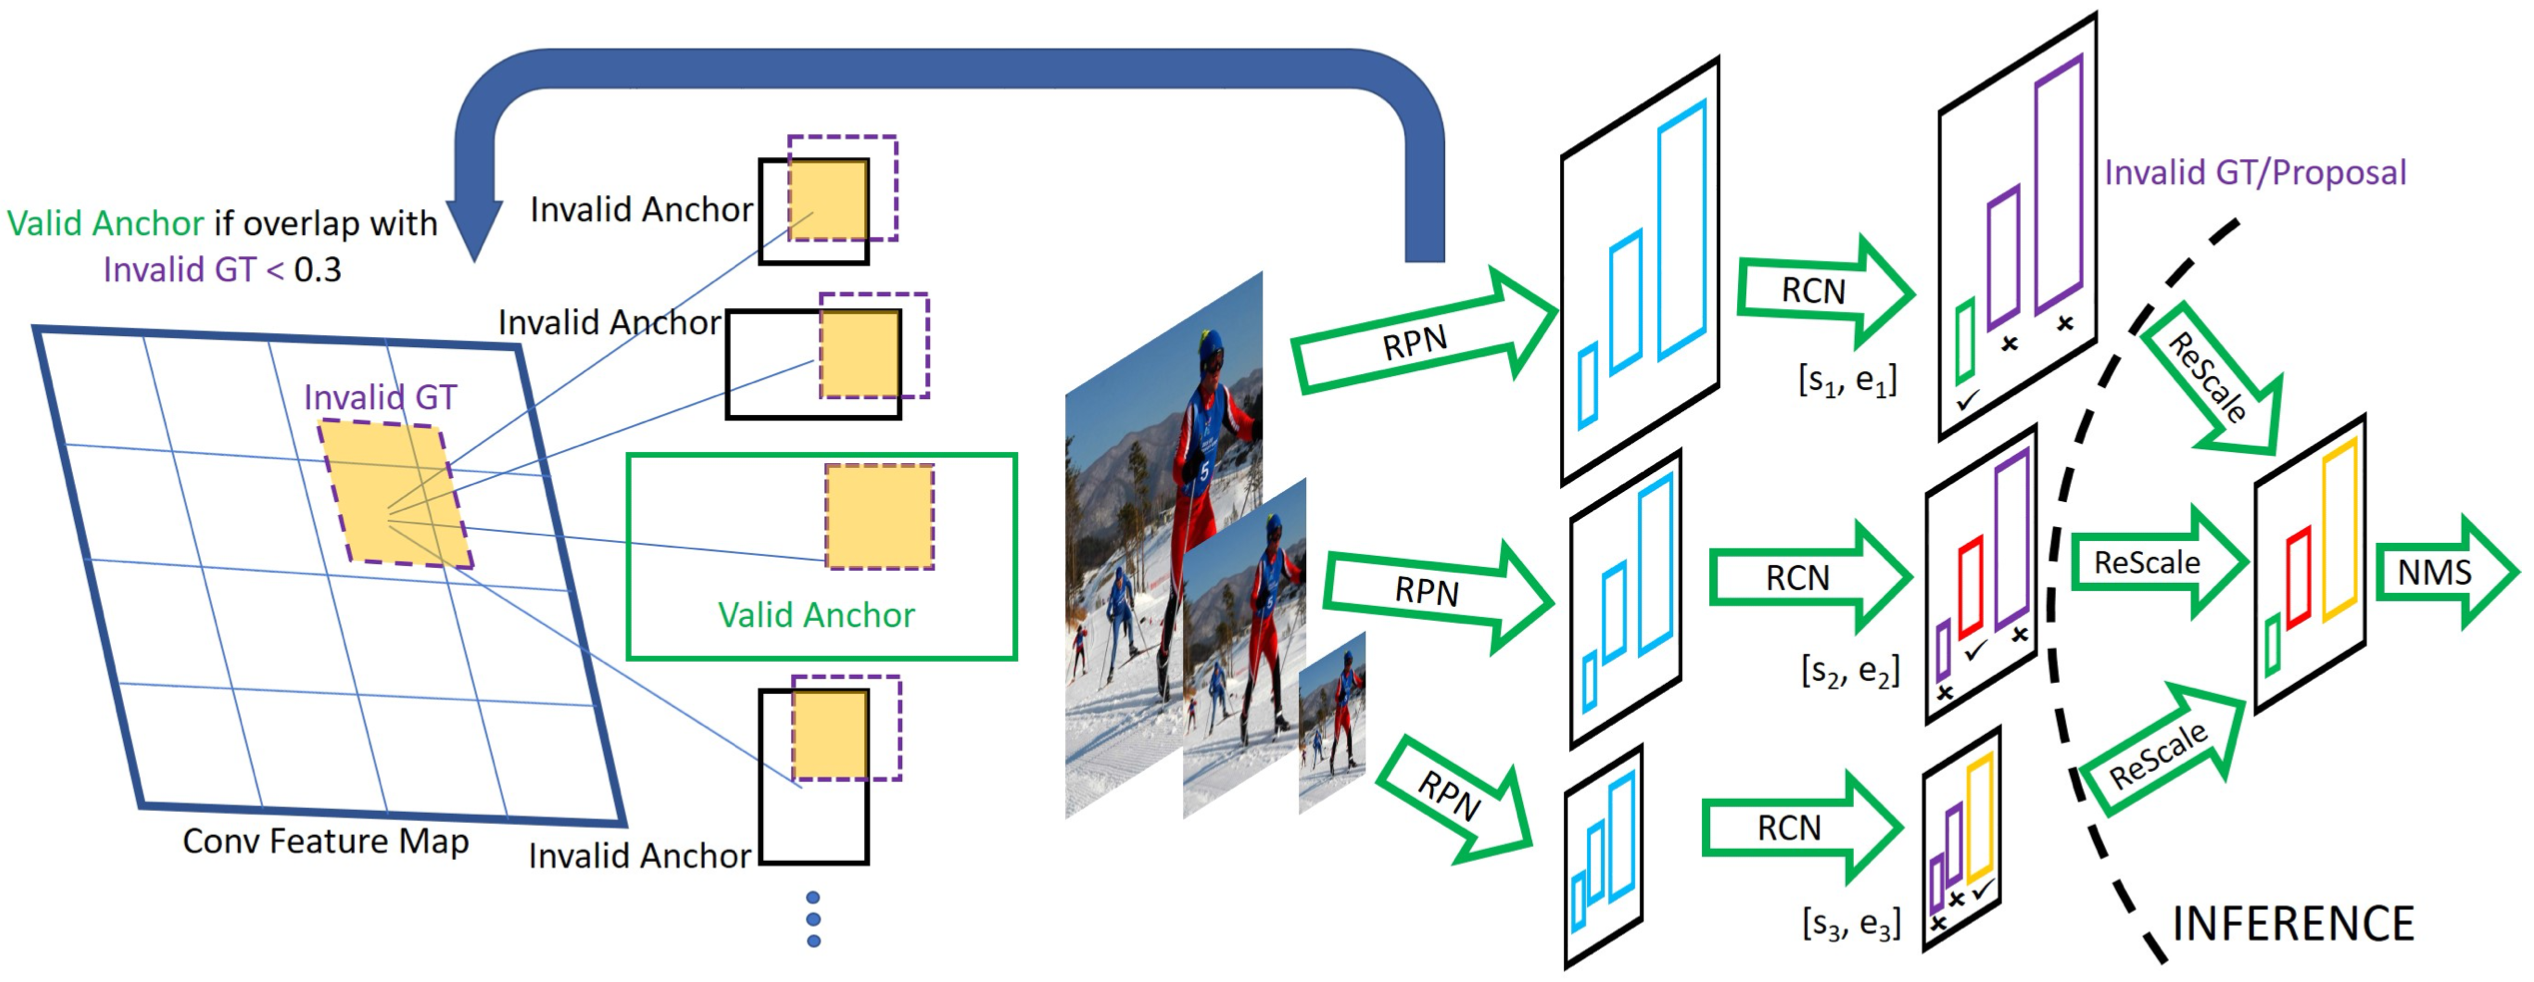
\includegraphics[width=16cm] {images/snip_model}
        \caption{Chi tiết kiến trúc mô hình SNIP trong quá trình train và test (Nguồn: \cite{singh2018analysis})}
        \label{fig:snip_model}
    \end{figure}

    \subsubsection{Kết quả của mô hình SNIP}
    \subsubsection{Vấn đề tồn đọng của mô hình SNIP}
    Tuy rằng đã có những cải thiện trong kết quả của mô hình SNIP, nhưng theo \cite{singh2018sniper}, mô hình SNIP vẫn tồn đọng vấn đề.
    Việc mô hình SNIP loại bỏ các object lớn khi kích thước ảnh được tăng lên khiến lãng phí chi phí tính toán trong quá trình train.
    Cụ thể hơn, khi một ảnh đuợc tăng kích thước lớn lên, và một object nào đó cũng có kích thước lớn và bị loại bỏ trong quá trình train, nhưng các lớp conv vẫn phải trượt qua các phần này trên ảnh và dẫn đến sự lãng phí tài nguyên tính toán.
    Hơn nữa, một trường hợp khác cũng gây lãng phí chi phí tính toán, đó là khi một ảnh có kích thước lớn nhưng cũng chỉ chứa các object lớn, khi ảnh này được tăng kích thước lên thì hiển nhiên các object lớn đó cũng bị loại bỏ.
    Việc lớp conv phải trượt qua một ảnh có kích thước lớn nhưng lại không có object nào trong ảnh đó được sử dụng để mô hình học (mô hình chỉ học được background trong trường hợp này) chắc chắn là một sự lãng phí.

    \subsection{Mô hình SNIPER}
    Xuất phát từ những vấn đề tồn đọng của mô hình SNIP, nhóm tác giả \cite{singh2018sniper} đã đề xuất mô hình Scale Normalization for Image Pyramids with Efficient Resampling (gọi tắt là SNIPER).
    Mô hình SNIPER hướng đến việc giảm thiểu đến tối đa khối lượng tính toán dư thừa từ đó tăng tốc được quá trình train mô hình.
    Nhóm tác giả đã thành công trong việc duy trì được kết quả mà mô hình SNIP đạt được trong khi SNIPER chỉ cần xử lý số lượng pixel ảnh bằng một phần ba số pixel mà SNIP phải xử lý.
    Điều này giúp việc train mô hình SNIPER tiết kiệm bộ nhớ hơn và có thể sử dụng được batch size lớn hơn trong quá trình train.
    \subsubsection{Ý tưởng của mô hình SNIPER}
    Nhằm tối ưu hoá khối lượng tính toán trong quá trình train, thay vì việc thay đổi kích thước của ảnh và chọn ra những object có kích thước phù hợp trong quá trình train, mô hình SNIPER cung cấp một cơ chế tiền xử lý dữ liệu.
    Từ bộ dữ liệu gốc ban đầu, các thuật toán của mô hình SNIPER xử lý và tạo ra bộ dữ liệu mới với các ảnh trong bộ dữ liệu được gọi là các Chip.
    \textbf{\textit{Định nghĩa Chip và phương pháp sinh ra Chip trong mô hình SNIPER}} \\
    Với ý tưởng loại bỏ những pixel dư thừa trên ảnh nhằm giảm khối lượng tính toán, Chip trong mô hình SNIPER có thể được hiểu là một phần của bức ảnh và đây cũng là đơn vị dữ liệu sử dụng trong quá trình train mô hình.
    Các bước sinh ra bộ Chip trong mô hình SNIPER như sau: \\
    \textit{Bước 1}: Nhóm tác giả định nghĩa một danh sách các kích thước ảnh {${s}_{1}$, ${s}_{2}$, ..., ${s}_{i}$, ..., ${s}_{n}$}. \\
    \textit{Bước 2}: SNIPER thay đổi kích thước của từng ảnh gốc ban đầu về từng kích ${s}_{i}$ trong danh sách trên.
    Ta thu được một bộ dữ liệu ảnh mới, trong đó, mỗi ảnh trong bộ dữ liệu ảnh ban đầu tương ứng với n ảnh với các kích thước khác nhau trong bộ dữ liệu ảnh mới. \\
    \textit{Bước 3}: Trên mỗi ảnh trong bộ dữ liệu ảnh mới, SNIPER đặt các ô vuông có kích thước \textit{KxK} sao cho tâm của các ô vuông này cách đều nhau một khoảng \textit{d} pixel. \\
    \textit{Bước 4}: SNIPER cắt ảnh theo các ô vuông đã đặt từ bước 3 để tạo thành các Chip. Danh sách các Chip này sẽ được lựa chọn và xử lý ở các thuật toán tiếp theo. \\

    \noindent
    \textbf{\textit{Phương pháp lựa chọn các Positive Chips}} \\
    Từ danh sách các Chip đã được tạo ra bởi thuật toán trên, nhóm tác giả thực hiện thuật toán lựa chọn các Positive Chips (Positive Chip Selection).
    Positive Chip ở đây được hiểu là các Chip chứa các groundtruth bounding box của object mà mô hình cần học.
    Các bước lựa chọn ra Positive Chip trong mô hình SNIPER như sau: \\
    \textit{Bước 1}: Nhóm tác giả định nghĩa một danh sách các khoảng kích thước bounding box phù hợp tương ứng với mỗi kích thước ảnh {${s}_{1}$, ..., ${s}_{n}$}.
    Cụ thể, với kích thước ảnh ${s}_{i}$, ta định nghĩa khoảng kích thước bounding box phù hợp ${R}^{i} = [{r}_{min}^{i}, {r}_{max}^{i}]$. \\
    \textit{Bước 2}: SNIPER kiểm tra từng bounding box trong từng Chip trên từng kích thước ảnh.
    Những bounding box có kích thước nằm trong khoảng kích thước phù hợp ${R}^{i}$ được thêm vào danh sách các bounding box hợp lệ ${G}^{i}$. \\
    \textit{Bước 3}: SNIPER lựa chọn các Chip từ danh sách các Chip ở thuật toán trên sao cho số lượng bounding box hợp lệ và nằm hoàn toàn trong một Chip là nhiều nhất.
    Danh sách các Positive Chips trên mỗi ảnh trong cùng một kích thước được gọi là ${C}_{pos}^{i}$. \\
    Một groundtruth bounding box bất kỳ sẽ luôn có một Chip nào đó chứa nó, một groundtruth bounding box bất kỳ có thể xuất hiện ở nhiều hơn một Chip và một groundtruth bounding box bất kỳ cũng có thể xuất hiện ở nhiều kích thước ảnh khác nhau.

    \subsubsection{Phương pháp lựa chọn các Negative Chips}
    \subsubsection{Cách gán nhãn cho các bounding box}
    \subsubsection{Kết quả của mô hình SNIPER}
    \subsubsection{Vấn đề tồn đọng của mô hình SNIPER}

    \subsection{Giới thiệu mô hình AutoFocus}
    \subsubsection{Ý tưởng của mô hình AutoFocus}
    \subsubsection{Thuật toán Focus Pixel}
    \subsubsection{Thuật toán sinh Focus Chips}
    \subsubsection{Thuật toán Focus Stacking}
    \subsubsection{Kết quả của mô hình AutoFocus}
}